% Die Optionen 'listof=totoc,bibliography=totoc' geben das Tabellen- und Abkürzungsverzeichnis im Inhaltsverzeichnis (toc Table of Content) aus. 
% \documentclass[12pt,oneside,titlepage,listof=totoc,bibliography=totoc]{scrartcl}
\documentclass[12pt,oneside,titlepage]{scrartcl}

\newcommand{\myAutor}{Henner Schmidt-Mustermann} % Autor
\newcommand{\myAdresse}{Hauptstra\ss e 123 \\ \> \> \> 57072 Musterstadt} % Adresse
\newcommand{\myTitel}{Nutzbarkeit und Effizienz von Latex-Vorlagen - Ein Proof of Conept für FOM Studenten} % Titel der Arbeit
\newcommand{\myBetreuer}{Prof. Dr. Karl-Heinz Backenzahn-Mustermann} % Betreuer
\newcommand{\myLehrveranstaltung}{Fallstudie/Wissenschaftliches Arbeiten} % Lehrveranstaltung
\newcommand{\myMatrikelNr}{543210} % Matrikelnummer
\newcommand{\myOrt}{Musterdorf} % Ort
\newcommand{\myAbgabeDatum}{\today} % Datum der Abgabe
\newcommand{\mySemesterZahl}{1} % Semesterzahl
\newcommand{\myHochschulName}{FOM Hochschule für Oekonomie \& Management Essen} % Name der Hochschule
\newcommand{\myHochschulStandort}{Siegen} % Standort der Hochschule
\newcommand{\myStudiengang}{Wirtschaftsinformatik} % Studiengang
\newcommand{\myThesisArt}{Seminararbeit} % Art der Arbeit
\newcommand{\myAkademischerGrad}{Bachelor of Science (B. Sc.)} % Zu erlangender akademische Grad
\newcommand{\myFirma}{Mustermann GmbH} % Firma

\usepackage[ngerman]{babel}
\selectlanguage{ngerman}
\usepackage[babel,german=quotes]{csquotes}

\usepackage[utf8]{luainputenc}
\usepackage[T1]{fontenc}
\usepackage{fancyhdr}
\usepackage{fancybox}
\usepackage[a4paper, left=4cm, right=2cm, top=4cm, bottom=2cm]{geometry}
\usepackage{graphicx}
\usepackage{colortbl}
\usepackage[capposition=top]{floatrow}
\usepackage{array}
\usepackage{float}      %Positionierung von Abb. und Tabellen mit [H] erzwingen
\usepackage{footnote}
\usepackage[singlelinecheck=false, labelfont=bf, font=bf]{caption} % Tabellendesign lt. Leitfaden
\usepackage{caption}
\usepackage{enumitem}
\usepackage{amssymb}
\usepackage{mathptmx}
\usepackage[scaled=0.9]{helvet} 
\usepackage{courier}
\usepackage{amsmath}
\usepackage[table]{xcolor}
\usepackage{marvosym}			% Verwendung von Symbolen, z.B. perfektes Eurozeichen
\usepackage[colorlinks=true,linkcolor=black]{hyperref}
\definecolor{darkblack}{rgb}{0,0,0}
\hypersetup{colorlinks=true, breaklinks=true, linkcolor=darkblack, menucolor=darkblack, urlcolor=darkblack}
\renewcommand\familydefault{\sfdefault}
\usepackage{ragged2e}

\usepackage[hang, multiple]{footmisc} % Mehrere Fussnoten nacheinander mit Komma separiert
\setlength{\footnotemargin}{1em}

%\usepackage{todonotes} % todo Aufgaben als Kommentare verfassen für verschiedene Editoren

\usepackage{epstopdf} %Pakete für Tabellen
\usepackage{nicefrac} % Brüche
\usepackage{multirow}
\usepackage{rotating} % vertikal schreiben
\usepackage{mdwlist}
\usepackage{tabularx}% für breitenangabe

\definecolor{dunkelgrau}{rgb}{0.8,0.8,0.8}
\definecolor{hellgrau}{rgb}{0.0,0.7,0.99}
% Colors for listings
\definecolor{mauve}{rgb}{0.58,0,0.82}
\definecolor{dkgreen}{rgb}{0,0.6,0}

\usepackage{listings} % sauber formatierter Quelltext
% JavaScript als Sprache definieren:
\lstdefinelanguage{JavaScript}{
	keywords={break, super, case, extends, switch, catch, finally, for, const, function, try, continue, if, typeof, debugger, var, default, in, void, delete, instanceof, while, do, new, with, else, return, yield, enum, let, await},
	keywordstyle=\color{blue}\bfseries,
	ndkeywords={class, export, boolean, throw, implements, import, this, interface, package, private, protected, public, static},
	ndkeywordstyle=\color{darkgray}\bfseries,
	identifierstyle=\color{black},
	sensitive=false,
	comment=[l]{//},
	morecomment=[s]{/*}{*/},
	commentstyle=\color{purple}\ttfamily,
	stringstyle=\color{red}\ttfamily,
	morestring=[b]',
	morestring=[b]"
}

\lstset{
	%language=JavaScript,
	numbers=left,
	numberstyle=\tiny,
	numbersep=5pt,
	breaklines=true,
	showstringspaces=false,
	frame=l ,
	xleftmargin=5pt,
	xrightmargin=5pt,
	basicstyle=\ttfamily\scriptsize, 
	stepnumber=1,
	keywordstyle=\color{blue},          % keyword style
  	commentstyle=\color{dkgreen},       % comment style
  	stringstyle=\color{mauve}         % string literal style
}

%%%% APA START / Biblatex
%% Zitierung und Literaturverzeichnis nach APA:
% Prof wünscht APA. Andere hatten das Problem auch schon...
% https://tex.stackexchange.com/questions/452228/modifying-bibliography-with-biblatex-biber-apa-style-locationpublisherdoi 
% https://texwelt.de/fragen/2686/wie-formatiere-ich-ein-bibtex-literaturverzeichnis-fur-eine-deutschsprachige-ausgabe-nach-den-regeln-der-apa


% Nötige Daten für Zitationen im Textteil: Nachnamen, Erscheinungsjahre, Besonderheiten: 
%  - Bei mehr als 6 Autoren: immer nur 1. Autor und "et al."
%  - Bei 3 bis 6 Autoren: Beim 1. nennen alle Nachnamen, danach nur noch 1. Autor und "et al."
%  - Bei zwei Autoren, Nennung beider
%  - Trennzeichen: Immer Komma, letzte Nachnamen mit "und", bsp: (Müller, Meier, Weber und Schmidt, 2018)

% Nötige Daten für Literaturverzeichnis:
% -  Internetquellen: (@online) 	Name Herausgeber Seite (analog Autor), 	Erscheinungsjahr, URL, Abrufdatum-URL
% -  Buch:(@book)				 Autoren,			 Erscheinungsjahr, Titel, ggfls. Hinweis auf Auflage/Band, Verlagsort, Verlagsname
% -  Zeitschriftenartikel(@article)   Autoren,			 Erscheinungsjahr, Titel des Artikel, Titel der Zeitschrift, Ausgabe mit Band- ggfls. Heftnummer, Seitenzahl(en)
% Weitere möglich, bisher keine Nutzung: Dissertationen (@phdthesis), Herausgeberwerk (@incollection), Buchkapitel- oder beitrag(@inbook)

\usepackage[
    style           = apa6,
    citestyle       = authoryear,
    citetracker     = false,    
    uniquelist      = false,    
    sorting         = nyt,
    sortcites       = true,
    autocite        = inline,
    maxbibnames     = 99,
    maxcitenames    = 6,
    backend         = biber,
    bibliography    = totoc,
    isbn            = true,
    doi             = true,
    urldate         = short
	]{biblatex}
	

	\hypersetup{hidelinks}  %Grüne Links auf Literaturverz. unterdrücken.
	\renewcommand*{\nameyeardelim}{\addcomma\space} % Bei Zitaten im Text Komma einfügen zw. Name und Jahr
	
	\setlength\bibitemsep{1.3ex} % Abstände im Literaturverzeichnis erhöhen
	\setlength\bibnamesep{1.0ex}

	\DeclareFieldFormat[online]{urldate}{[#1\printfield{urldate}].} % Anpassung @online Bibl: Datum in eckigen Klammern ans Ende
	\DeclareFieldFormat[online]{title}{\mkbibemph{#1}} %Titel Kursiv

	%\DeclareFieldFormat[online]{autor}{#1\nopunct{autor}} % Ohne Punkt am Ende -funktionslos!!- TODO: Punkt entfernen

	%\DeclareFieldFormat[online]{url}{Verfügbar unter\space \url{#1}} % Anpassung @online Text vor URL
	%\renewbibmacro*{url+urldate}{\usebibmacro{url}\ifentrytype{online}\setunit*{\addspace}\usebibmacro{urldate}} % Fehler: Hiermit tauchen bei allen anderen Arten * am Ende auf!

%%%% APA ENDE

\addbibresource{literatur.bib} %Bib-Datei einbinden
\nocite{*} % Die folgende Zeile trägt ALLE Werke aus literatur.bib in das Verz. ein, auskommentieren um nur die anzuzeigen, die zitiert wurden
\AtBeginBibliography{\singlespacing} % Zeilenabstand im Literaturverzeichnis ist Einzeilig - siehe Leitfaden S. 14

\usepackage{hyphsubst} %Silbentrennung
\HyphSubstIfExists{ngerman-x-latest}{%
\HyphSubstLet{ngerman}{ngerman-x-latest}}{}

\graphicspath{{./}{./media/}} % Pfad fuer Abbildungen

\usepackage{titletoc} % Weitere Ebene einfügen
\makeatletter

% Setze die Tiefe des Inhaltsverzeichnis auf 4 Ebenen -  Damit erscheinen \paragraph-Sektionen auch im Inhaltsverzeichnis
\setcounter{secnumdepth}{4}
\setcounter{tocdepth}{4}

% Fuege Abstand nach unten wie in einer normalen \section hinzu
\renewcommand{\paragraph}{%
  \@startsection{paragraph}{4}%
  {\z@}{3.25ex \@plus 1ex \@minus .2ex}{1.5ex plus 0.2ex}%
  {\normalfont\normalsize\bfseries\sffamily}%
}

\makeatother

\usepackage{appendix} % Paket für die Nutzung von Anhängen
\usepackage{setspace} % Zeilenabstand 1,5-zeilig
\onehalfspacing

\setlength{\parindent}{0mm} % Absätze durch eine neue Zeile
\setlength{\parskip}{0.8em plus 0.5em minus 0.3em}

\sloppy					%Abstände variieren
\pagestyle{headings}

\usepackage[printonlyused]{acronym} % Abkürzungsverzeichnis

% PDF Meta Daten setzen
\hypersetup{
    pdfinfo={
        Title={\myTitel},
        Subject={\myStudiengang},
        Author={\myAutor},
        Build=1.1
    }
}

% Umlaute in Code korrekt darstellen - siehe  https://en.wikibooks.org/wiki/LaTeX/Source_Code_Listings
\lstset{literate=
	{á}{{\'a}}1 {é}{{\'e}}1 {í}{{\'i}}1 {ó}{{\'o}}1 {ú}{{\'u}}1
	{Á}{{\'A}}1 {É}{{\'E}}1 {Í}{{\'I}}1 {Ó}{{\'O}}1 {Ú}{{\'U}}1
	{à}{{\`a}}1 {è}{{\`e}}1 {ì}{{\`i}}1 {ò}{{\`o}}1 {ù}{{\`u}}1
	{À}{{\`A}}1 {È}{{\'E}}1 {Ì}{{\`I}}1 {Ò}{{\`O}}1 {Ù}{{\`U}}1
	{ä}{{\"a}}1 {ë}{{\"e}}1 {ï}{{\"i}}1 {ö}{{\"o}}1 {ü}{{\"u}}1
	{Ä}{{\"A}}1 {Ë}{{\"E}}1 {Ï}{{\"I}}1 {Ö}{{\"O}}1 {Ü}{{\"U}}1
	{â}{{\^a}}1 {ê}{{\^e}}1 {î}{{\^i}}1 {ô}{{\^o}}1 {û}{{\^u}}1
	{Â}{{\^A}}1 {Ê}{{\^E}}1 {Î}{{\^I}}1 {Ô}{{\^O}}1 {Û}{{\^U}}1
	{œ}{{\oe}}1 {Œ}{{\OE}}1 {æ}{{\ae}}1 {Æ}{{\AE}}1 {ß}{{\ss}}1
	{ű}{{\H{u}}}1 {Ű}{{\H{U}}}1 {ő}{{\H{o}}}1 {Ő}{{\H{O}}}1
	{ç}{{\c c}}1 {Ç}{{\c C}}1 {ø}{{\o}}1 {å}{{\r a}}1 {Å}{{\r A}}1
	{€}{{\EUR}}1 {£}{{\pounds}}1 {„}{{\glqq{}}}1
}

\pagestyle{fancy} % Kopfbereich / Header definieren
\fancyhf{} % Seitenzahl oben, mittig, mit Strichen beidseits: \fancyhead[C]{-\ \thepage\ -}

\fancyhead[C]{\thepage} % Seitenzahl oben, mittig, entsprechend Leitfaden ohne Striche beidseits
\renewcommand{\headrulewidth}{0.4pt} % Waagerechte Linie unterhalb des Kopfbereiches anzeigen. Alternativ weg: \renewcommand{\headrulewidth}{0pt}

\begin{document} % Start the document here:

\pagenumbering{Roman}								% Seitennumerierung auf römisch umstellen
\renewcommand{\refname}{Literaturverzeichnis}		% "Literatur" in "Literaturverzeichnis" umbenennen
\newcolumntype{C}{>{\centering\arraybackslash}X}	% Neuer Tabellen-Spalten-Typ: Zentriert und umbrechbar

\begin{titlepage} % Titlepage/Deckblatt
	\newgeometry{left=2cm, right=2cm, top=2cm, bottom=2cm}
	\begin{center}
		\textbf{\myHochschulName}\\
		\textbf{Hochschulzentrum \myHochschulStandort}\\
		\vspace{1.5cm}
			
\includegraphics[width=3cm]{media/fomLogo} \\
		\vspace{1.5cm}
		Berufsbegleitender Studiengang\\
		\myStudiengang, \mySemesterZahl. Semester\\
		\vspace{2cm}
		\textbf{\myThesisArt}\\
		%\textbf{zur Erlangung des Grades eines	}\\
		%\textbf{\myAkademischerGrad}\\
		% Oder für Hausarbeiten:
		\textbf{im Rahmen der Lehrveranstaltung}\\
		\textbf{\myLehrveranstaltung}\\
		\vspace{2cm}
		über das Thema\\
		\Large{\myTitel}\\
		\vspace{0.2cm}
	\end{center}
	\normalsize
	\vfill
	\begin{tabbing}
		Links \= Mitte \=Mittez \= Rechts\kill
		Betreuer: \> \> \>\myBetreuer\\
		\> \> \\
		Autor: \> \> \> \myAutor\\
		\> \> \>  Matrikelnr.: \myMatrikelNr\\
		\> \> \> \myAdresse\\
		\> \> \>  \\
		Abgabe: \> \> \> \myAbgabeDatum
	\end{tabbing}
\end{titlepage}

%-------Ende Titelseite-------------


% Sperrvermerk
%\newpage
%\thispagestyle{empty}
%\section*{Sperrvermerk}
%Die vorliegende Abschlussarbeit mit dem Titel \enquote{\myTitel} enthält unternehmensinterne Daten der Firma \myFirma . Daher ist sie nur zur Vorlage bei der FOM sowie den Begutachtern der Arbeit bestimmt. Für die Öffentlichkeit und dritte Personen darf sie nicht zugänglich sein.
%\par\medskip
%\par\medskip
%\_\_\_\_\_\_\_\_\_\_\_\_\_\_\_\_\_\_\_\_\_\_\_\_ \hspace{1.5cm} \_\_\_\_\_\_\_\_\_\_\_\_\_\_\_\_\_\_\_\_\_\_\_\_ \\
%(Ort, Datum)\hspace{4.5cm}
%(Eigenhändige Unterschrift)
%\newpage


% Inhaltsverzeichnis
\setcounter{page}{2}
\addtocontents{toc}{\protect\enlargethispage{-20mm}}
\clearpage
\tableofcontents
\newpage
\setcounter{tocdepth}{2} %wurde  in zusaetzlichesMaterial.tex auf 0 gesetzt um Inhalt des Anhangs zu verbergen. Dadurch gehen allerdings Abbildungs und Tabellenverzeichnis kaputt.

\listoffigures % Abbildungsverzeichnis
\newpage

\listoftables % Tabellenverzeichnis
\newpage

% \addcontentsline{toc}{section}{Abkürzungsverzeichnis} % Falls das Abkürzungsverzeichnis im Inhaltsverzeichnis angezeigt werden soll einkommentieren.
\section*{Abkürzungsverzeichnis} % Abkürzungsverzeichnis

\begin{acronym}[WYSIWYG]\itemsep0pt %der Parameter in Klammern sollte die längste Abkürzung sein. Damit wird der Abstand zwischen Abkürzung und Übersetzung festgelegt
  \acro{OC}{FOM Online Campus}
  \acro{WYSIWYG}{What you see is what you get}
  \acro{Beispiel}{Nicht verwendet, taucht nicht im Abkürzungsverzeichnis auf}
\end{acronym}
\newpage

\pagenumbering{arabic} % Seitennummerierung auf arabisch und ab 1 beginnend umstellen
\setcounter{page}{1}

\section{Einleitung} % Kapitel / Inhalte
Dies soll eine \LaTeX{}-Vorlage für den persönlichen Gebrauch werden. Sie hat weder einen Anspruch auf Richtigkeit, noch auf Vollständigkeit. Die Quellen liegen auf Github zur allgemeinen Verwendung. Verbesserungen sind jederzeit willkommen.

\subsection{Zielsetzung}
Kleiner Reminder für mich in Bezug auf die Dinge, die wir bei der Thesis beachten sollten und \LaTeX{}-Vorlage für die Thesis.

\subsection{Aufbau der Arbeit}
Kapitel \ref{infos} enthält die Inhalte des Thesis-Days und alles, was zum inhaltlichen erstellen der Thesis relevant sein könnte. In Kapitel \ref{latexDetails} \nameref{latexDetails} findet ihr wichtige Anmerkungen zu \LaTeX{}, wobei die wirklich wichtigen Dinge im Quelltext dieses Dokumentes stehen (siehe auch die Verzeichnisstruktur in Abbildung \ref{fig:verzeichnisStruktur}).


\begin{figure}[H]
\caption{Verzeichnisstruktur der \LaTeX{}-Datein}\label{fig:verzeichnisStruktur}

\includegraphics[width=0.9\textwidth]{verzeichnisStruktur}
\\
Quelle: Eigene Darstellung
\end{figure}


\newpage
\section{Informationen vom Thesis-Day} \label{infos}
Siehe auch Wissenschaftliches Arbeiten~ Damit sollten alle wichtigen Informationen abgedeckt sein ;-)

\subsection{Pre-Anmeldephase}
\subsubsection{Vorüberlegungen}
Trichtermethode: Man beginnt mit der eigentlichen  Konklusion und überlegt dann, welche allgemeinen Teile dafür benötigt werden.

Welchen Mehrwert soll die Arbeit bieten \footnote{Diese Fu\ss note hat inhaltlich keinen Sinn. Es soll nur ein langer Text generiert werden, dass dieser Vermerk über zwei Zeilen reicht und bündig dargestellt wird.}? Auch darüber nachdenken, wie die Arbeit einen selbst weiter bringen kann. Studienverlauf prüfen. Welche Vorlesungen hat mich besonders interessiert? Wo liegen meine Stärken etc.

\begin{enumerate}
\item Themenfindung
\item Literaturrecherche
\item Gliederung/Motivationspapier erstellen
\item Betreuerauswahl (siehe Liste im \ac{OC})
\item Anmeldung (ab 141 Credits möglich)
\end{enumerate}

\subsubsection{Anregungen finden}
\begin{itemize}
\item \href{http://www.diplom.de}{www.diplom.de}
\item \href{http://www.hausarbeiten.de}{www.hausarbeiten.de}
\item Datenbanken aus Tools and Methods
\item etc.
\end{itemize}

\newpage
\subsection{Anfertigungsphase}
Die Anmeldung ist mittlerweile jeden Mittwoch möglich.

Laut Herrn Keller sollte der Umfang der Thesis (für eine gute Note) eher im Bereich der 60 Seiten liegen. Wie immer ist das vermutlich mit dem Betreuer abzustimmen. Die Liste der Dozenten, die Abschlussarbeiten betreuen, findet sich auch im \ac{OC}.

Zeit zur Erstellung der Thesis 2-4 Monate.

Es müssen zwei gedruckte Arbeiten abgegeben werden. Flüchtige Quellen als PDF ausgeben lassen und auf CD abgeben. Thesis zusätzlich digital einreichen. Beim Binden der Thesis auf Qualität achten. Haptik und erster Eindruck sind in der Bewertung \enquote{auch} wichtig. Arbeiten können in jedem FOM Studienzentrum abgegeben werden.

\subsection{Post-Abgabephase}
Nach Abgabe ca. 2 Wochen bis zum Kolloquium.

Kolloquium:
\begin{itemize}
\item Dauer: 30 Minuten
\item Präsentation (manche Prüfer wollen eine, andere nicht)
\item Betreuer vorher fragen was er möchte
\item Es gibt einen Frageteil, dieser bezieht sich auf die Arbeit, kann aber auch darüber hinaus gehen.
\item Der Tag des Kolloquiums steht auf der Endbenotung
\item Thesis und Kolloquium sind zwei getrennte Prüfungsbereiche. Für beide gibt es nur zwei Versuche.
\item Am Tag des Kolloquiums erhält man die Bestätigung, ob bestanden oder nicht
\end{itemize}


\newpage
\section{Latex-Details} \label{latexDetails}

\subsection{Verwendete Software, Editor und Zusatzpakete}
\subsubsection{Windows 8+}
\begin{itemize}
\item MikTex: 2.9, 32-bit
\item Biblatex: 3.5, Zusatz: Biber.exe
\item Editor: TexStudio (kann ich empfehlen), Notepad++
\end{itemize}

\subsubsection{Mac OSX und iOS}
\begin{itemize}
\item MacTeX: \url{https://tug.org/mactex}
\item Editor: TexPad \url{https://www.texpadapp.com}
\end{itemize}

\subsubsection{Online}
Overleaf ist eine Online-Anwendung mit der Ihr direkt im Browser an eurer Thesis schreiben könnt. Bis 1GB Größe und maximal 60 Einzeldateien könnt ihr Overleaf kostenlos nutzen: \url{https://www.overleaf.com/}


\subsection{Dokumentenklasse}
Eigentlich hatte Prof. Finke empfohlen die Dokumentklassen \enquote{Book} oder \enquote{Report} für die Erstellung der Bachelor-Thesis zu verwenden, da diese über weitere Gliederungsebenen verfügen. Ich verwende dennoch eine leicht modifizierte Komaskript-Klasse \enquote{scrartcl}, mit der Erweiterung um eine Ebene. Siehe (skripte/weitereEbene.tex). Das Skript stammt irgendwo aus den Netz und übersteigt meine \LaTeX{}-Fähigkeiten. Dadurch kann ich über eine weitere Ebene in der Arbeit verfügen, ohne mich mit der Modifikation von Kapitel-Seiten rumschlagen~zu müssen. Diese Quelle ist nur zur Demonstration und hat keinen inhaltlichen Bezug hierzu. Es werden übrigens nur die Quellen im Literaturverzeichnis angezeigt, die auch referenziert sind.


\subsection{Grafiken}
Das Paket \textbackslash usepackage\{float\} ermöglicht es die Grafiken und Tabellen an der Stelle im Text zu positionieren, wo diese im Quelltext stehen (Option H). Ansonsten würde \LaTeX{} diese dort unterbringen, wo es typographisch sinnvoll wäre - das wollen wir ja nicht ;-).

Die Breite der Grafiken am Besten relativ zum Text angeben.

\subsection{Quellcode}
Quellcode kann auf unterschiedliche Arten eingebaut werden.
Zum einen kann es hier durch direktives Einbinden in der Kapitel-Datei geschehen.
\begin{lstlisting}
% Hier wird aufgezeigt, wie man eine Grafik einbindet, es wird also in der PDF angezeigt,
% da es in einem Quellcode-Listing steht.
% Auch wenn es hier faelschlicherweise als LaTeX-Befehl angezeigt wird.
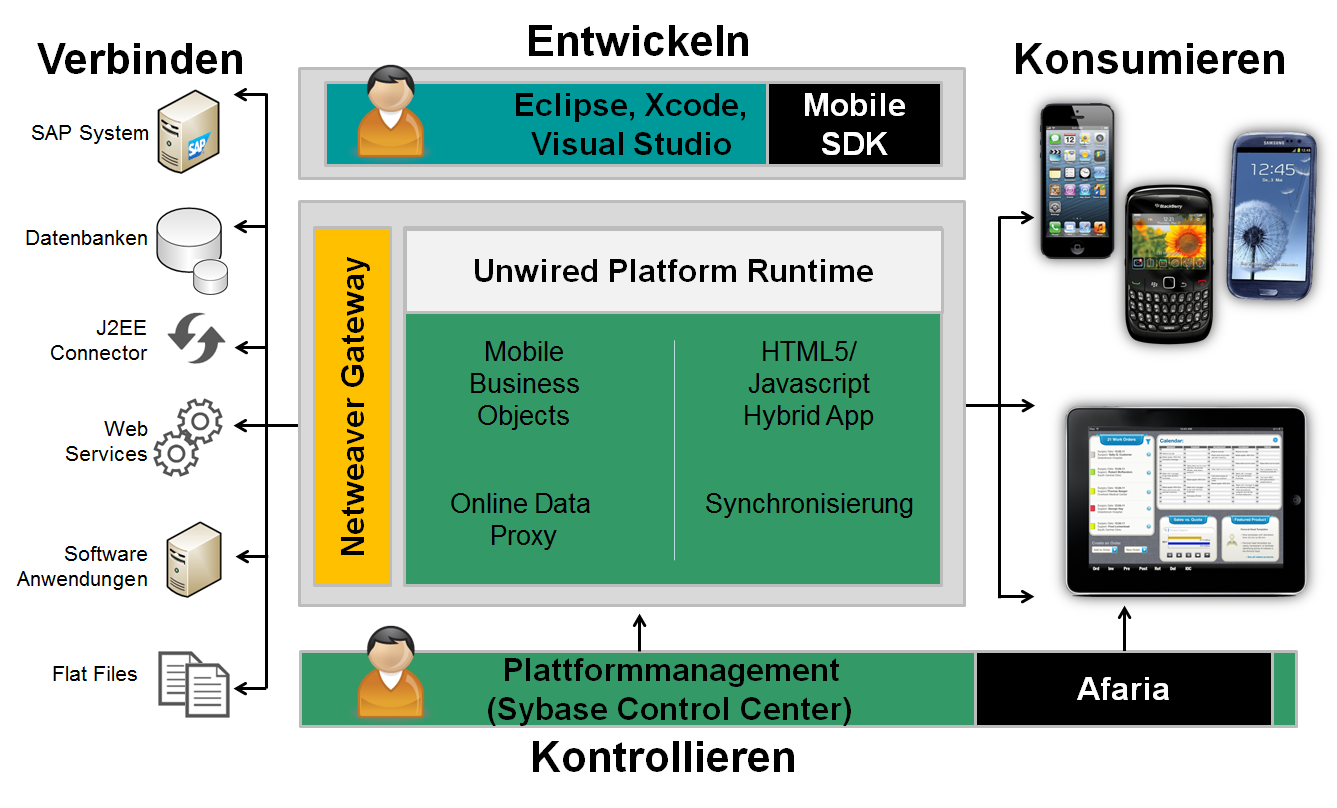
\includegraphics[width=0.9\textwidth]{sup}
\end{lstlisting}

Bei längeren Quellcode-Listings empfiehlt es sich jedoch auf eine externe Datei im Ordner Quellcode zu verlinken und diese einzubauen:
\lstinputlisting[language=HTML]{./media/beispiel.html}

Statt dem Package lstlisting, welches direkt auf Tex basiert, kann auch das Package minted verwendet werden.
Dieses Package basiert auf python-pygments und unterstützt weit mehr Sprachkonstrukte als lstlisting.
Um das Paket zu verwenden muss es eingebunden werden und zusätzlich python-pygments installiert sein.
(Dies ist mit im Dockerfile vorhanden. Für die anderen Compile-Methoden, wie das native verwenden von Tex Live findet sich hier die Installationsanleitung für das minted Paket: https://ctan.org/pkg/minted?lang=de)

Damit das kompilieren ohne Python trotzdem möglich ist, ist die Funktion standardmäßig ausgebaut. Deshalb muss zusätzlich in der Datei \begin{verbatim}thesis_main.tex \usepackage{minted} \end{verbatim} wieder einkommentiert werden. 

Minted lässt sich dann ganz ähnlich zu lstlisting verwenden:
\begin{lstlisting}
	\begin{minted}{c}
		int main() {
			printf("hello, world");
			return 0;
		}
	\end{minted}
\end{lstlisting}	

Da der Pfad zu den Abbildungen im Hauptdokument definiert wurde, muss hier nur noch der Name des Bildes ohne Dateiendung stehen (sup).

\begin{figure}[H]
\caption{Titel der Abbildung hier}
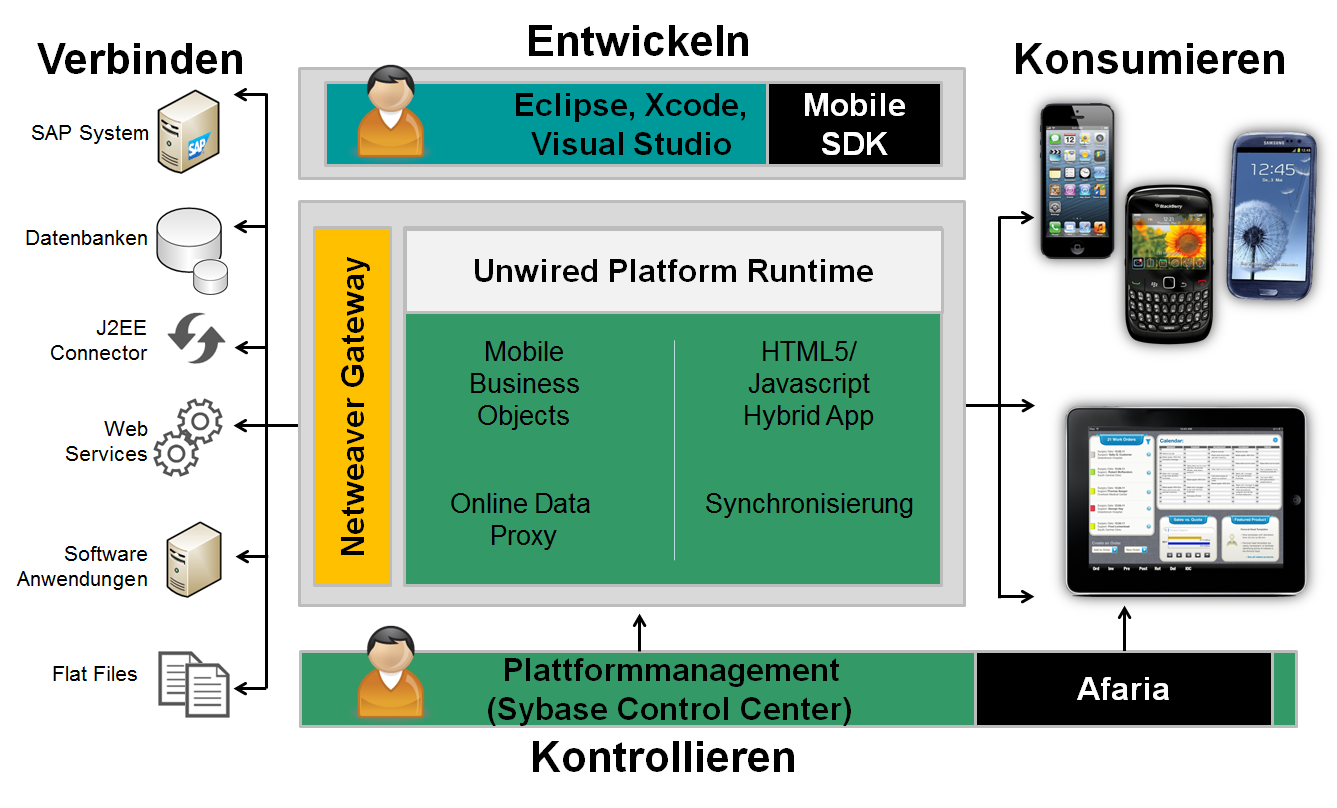
\includegraphics[width=0.9\textwidth]{sup}
\\ Quelle: Eigene Darstellung
\end{figure}

\subsection{Tabellen}
\begin{table}[H]
\caption{Beispieltabelle 1}
\label{tbl:beispieltabelle2}
\begin{tabularx}{\textwidth}[ht]{|l|X|l|}
  \hline
  \textbf{Abkürzung} & \textbf{Beschreibung} & \textbf{Berechnung}\\
  \hline\hline
    MEK & Materialeinzelkosten & \\
  	MGK & Materialgemeinkosten & $+ \uparrow$~*\\
    FEK & Fertigungseinzelkosten & \\
  	FGK & Fertigungsgemeinkosten & $+ \uparrow$~*\\
	SEKF & Sondereinzelkosten der Fertigung & \\
	\hline\hline
	\multicolumn{3}{|l|}{\textbf{= Herstellungskosten}} \\
	\hline\hline
  	VwGK & Verwaltungsgemeinkosten & $+ \uparrow$~*\\
  	VtGK & Vertriebsgemeinkosten & $+ \uparrow$~*\\
  	SEKVt & Sondereinzelkosten des Vertriebes & \\
	\hline\hline
	\multicolumn{3}{|l|}{\textbf{= Selbstkosten}} \\
	\hline\hline
	\multicolumn{3}{|l|}{+ Gewinnaufschlag} \\
	\multicolumn{3}{|l|}{+ Rabatte} \\
	\hline\hline
	\multicolumn{3}{|l|}{\textbf{= Nettoverkaufspreis (NVP)}} \\
	\hline
	\multicolumn{3}{|l|}{+ Umsatzsteuer} \\
	\hline\hline
	\multicolumn{3}{|l|}{\textbf{= Bruttoverkaufspreis (BVP)}} \\
	\hline
\end{tabularx} \\
\cite[Quelle: In Anlehnung an][S. 4]{FOM}
\end{table}

%\clearpage % hiermit werden alle Bilder Tabellen ausgeworfen

\subsection{Biblatex}
Von den vielen verfügbaren Literatur-Paketen habe ich mich für Biblatex entschieden. Die Anforderungen der FOM sollten hiermit erfüllt sein. Ich habe bisher nur Einträge \enquote{@book} getestet. Wie immer steckt der Teufel hier im Detail und es wird sich später herausstellen, ob Biblatex eine gute Wahl war. Die Anpassungen hierfür liegen unter skripte/modsBiblatex. Ich verwende das Backend Biber, welches bib-Dateien in UTF-8 verarbeiten kann.

In der für den Leitfaden 2018 aktualisierten Version sind außerdem Beispiele für \enquote{online},also Webseiten, und \enquote{article}, also wissenschaftliche Artikel, enthalten.

Laut Leitfaden sollen maximal 3 Autoren genannt werden und danach mit
\enquote{et. al.} bzw. \enquote{u.a.} ergänzt werden. Damit im Literaturverzeichnis auch nur max.
3 Autoren stehen, muss man beim Füllen der literatur.bib-Datei darauf achten auch nur 3
einzutragen. Weitere Autoren kann man einfach mit \enquote{and others} ergänzen.
Siehe Eintrag für \enquote{Balzert.2008}. Zitiert man dann diese Werk, werden auch in
der Fussnote alle Autoren korrekt genannt wie in dieser
Fußnote\cite[Vgl.][S.1]{Balzert7} zu sehen ist.\\
Hat man dagegen mehr als 3 Autoren in der bib-Datei hinterlegt, stehen im
Literaturverzeichnis alle drin. In der Fussnote dagegen, steht nur
einer\parencite[][S. 1]{becker2016hrsg}, was dem Leitfaden widerspricht.\\
Die Anzahl von 3 wird übrigens über die Option \enquote{maxcitenames=3} des
biblatex-Packages gesetzt. Man muss selbst schauen, dass die Anzahl der Autoren
in den Bib-Dateien mit der Optionseinstellung übereinstimmt.

Diese Fussnote soll zeigen, wie mit einem \enquote{von} vor dem Namen des Autors
umgegangen wird\parencite{Lucke2018hrsg}. Man muss für die korrekte
Sortierung eines solchens Namens im Literaturverzeichnis einen \enquote{sortkey}


\subsubsection{APA Richtlinien}

Einige Doezenten verlagen die Zitierungen und das Literaturverzeichnis nach den APA Richtlininen. Daher nun ein ganzer Block an Test-Zitaten... (\cite{Belastingdienst}) und \cite{Decker2009} sowie \citeyear{Belastingdienst} sowie \citeyear{Decker2009}.

Außerdem gibt es \parencite{Wiederhofer2017} und \parencite{Decker2009} sowie \citeauthor{Wiederhofer2017} und \citeauthor{Lucke2018hrsg}.

Weiter noch textcite mit \textcite{FOM} und \textcite{Wiederhofer2017} sowie \textcite{Decker2009}. Darin sollten mehrere Autoren mit dem Wort 'und' verbunden sein. 

Auch mehrere Autoren sind möglich APA konform zu bennen mit \parencite{Balzert7,Decker2009,Wiederhofer2017}.

Hier noch versuche mit Seitenzahlen: Wiedenhofer z.B: \parencite[5]{Wiederhofer2017}.

Es fehlt noch das Komma zwischen dem Nam en und dem Jahr. Noch ein versuch, hier mit Beckert \citeauthor{Beckert3}. 
Nun tests mit Struktur:\\
Sieben Autoren mit cite \cite{Balzert7}\\
mit textcite \textcite{Balzert7}\\
und mit parenite \parencite{Balzert7}\\
außerdem nur mit citeauthor \citeauthor{Balzert7} und citeyear \citeyear{Balzert7}.\\
\\
Drei Autoren mit cite \cite{Beckert3}\\
mit textcite \textcite{Beckert3}\\
und mit parenite \parencite{Beckert3}\\
außerdem nur mit citeauthor \citeauthor{Beckert3} und citeyear \citeyear{Beckert3}.\\
\\
Drei Autoren und 2. Aufruf mit cite \cite{Beckert3}\\
mit textcite \textcite{Beckert3}\\
und mit parenite \parencite{Beckert3}\\
außerdem nur mit citeauthor \citeauthor{Beckert3} und citeyear \citeyear{Beckert3}.\\
\\
Zwei Autoren mit cite \cite{Tanenbaum2}\\
mit textcite \textcite{Tanenbaum2}\\
und mit parenite \parencite{Tanenbaum2}\\
außerdem nur mit citeauthor \citeauthor{Tanenbaum2} und citeyear \citeyear{Tanenbaum2}.\\
\\
Ein Autor mit cite \cite{Beckert1}\\
mit textcite \textcite{Beckert1}\\
und mit parenite \parencite{Beckert1}\\
außerdem nur mit citeauthor \citeauthor{Beckert1} und citeyear \citeyear{Beckert1}.\\
\\
\\
\\
Außerdem noch ein Aritkel mit Seitenzahlen\\
Sieben Autoren mit cite \cite{Wiederhofer2017}\\
mit textcite \textcite{Wiederhofer2017}\\
und mit parenite \parencite{Wiederhofer2017}\\
außerdem nur mit citeauthor \citeauthor{Wiederhofer2017} und citeyear \citeyear{Wiederhofer2017}.\\



\subsection{Abkürzungen}
Abkürzungen werden mithilfe des Pakets Acronym eingebunden. Alle Abkürzungen sollten in der Datei acronyms.tex mithilfe des \begin{verbatim}
	\acro
\end{verbatim} Befehls festgelegt. Im Text werden diese dann mit \begin{verbatim}
	\ac{Abkürzung}
\end{verbatim} benutzt. Bei der ersten Verwendung einer Abkürzung wird der der Begriff in beiden Formen dargestellt. So wie hier: \ac{WYSIWYG}. Nur wenn eine Abkürzung tatsächlich verwendet wird erscheint sie auch im Abkürzungsverzeichnis.

Sollte es im Abkürzungsverzeichnis zu Anzeigefehlern kommen kann dies daher rühren, dass eine Abkürzung verwendet wird, die länger ist als \ac{WYSIWYG}. In diesem Fall müsst ihr in der Datei acronyms.tex den Parameter [WYSIWYG] durch eure längere Abkürzung ersetzen.

\subsection{Listen und Aufzählungen}
\subsubsection{Listen}
\begin{itemize}
\item ein wichtiger Punkt
\item noch ein wichtiger Punkt
\item und so weiter
\end{itemize}
\subsubsection{Aufzählungen}
\begin{enumerate}
\item Reihenfolge ist hier wichtig
\item Dieser Punkt kommt nach dem ersten
\item Da sollte jetzt eine 3 vorne stehen
\end{enumerate}

\paragraph{Tiefste Ebene 1}
Dies ist die tiefste Gliederungsebene. Sollten doch mehr Ebenen benötigt werden, muss eine andere Dokumentenklasse verwendet werden.

\paragraph{Tiefste Ebene 2}
Der zweite Punkt in dieser Ebene ist zur Erinnerung daran, dass es nie nie niemals nur einen Unterpunkt geben darf.

\subsection{Skript zum Kompilieren}
Latex will ja bekanntlich in einer bestimmten Reihenfolge aufgerufen werden:
\begin{lstlisting}
lualatex thesis_main.tex
biber thesis_main
lualatex thesis_main.tex
lualatex thesis_main.tex
thesis_main.pdf
\end{lstlisting}

Dies ist der Inhalt der Batchdatei \enquote{compile.bat}.
\section{Fazit}
Wünsche Euch allen viel Erfolg für das 7. Semester und bei der Erstellung der Thesis. Über Anregungen und Verbesserung an dieser Vorlage würde ich mich sehr freuen. 

\newpage % Anhang
\section*{Anhang} %Überschrift "Anhang", ohne Nummerierung
		\addcontentsline{toc}{section}{Anhang} %Den Anhang ohne Nummer zum Inhaltsverzeichnis hinzufügen

		\begin{appendices}
			\addtocontents{toc}{\protect\setcounter{tocdepth}{0}} %
				\renewcommand{\thesection}{Anhang \arabic{section}:}
				\renewcommand\thesubsection{Anhang \arabic{section}.\arabic{subsection}:}
	\section{Beispielanhang}\label{Beispielanhang}
			Dieser Abschnitt dient nur dazu zu demonstrieren, wie ein Anhang aufgebaut seien kann.
			\subsection{Weitere Gliederungsebene}
			Auch eine zweite Gliederungsebene ist möglich.
	\section{Bilder}
			Auch mit Bildern.
			Diese tauchen nicht im Abbildungsverzeichnis auf.
			\begin{figure}[H]
				\centering
				\caption[]{Beispielbild}
				\label{fig:Beispielbild}
				
\includegraphics[width=1\textwidth]{verzeichnisStruktur}
			\end{figure}

		\end{appendices}
		\addtocontents{toc}{\protect\setcounter{tocdepth}{2}}

\newpage % Literaturverzeichnis
	\printbibliography[heading=bibintoc,title=Literaturverzeichnis]
	\newpage

	\pagenumbering{gobble} % Keine Seitenzahlen mehr


\section*{Ehrenwörtliche Erklärung} % Ehrenwörtliche Erklärung
	Hiermit versichere ich, dass die vorliegende Arbeit von mir selbstständig und ohne unerlaubte Hilfe angefertigt worden ist, insbesondere dass ich alle Stellen, die wörtlich oder annähernd wörtlich aus Veröffentlichungen entnommen sind, durch Zitate als solche gekennzeichnet habe. Ich versichere auch, dass die von mir eingereichte schriftliche Version mit der digitalen Version übereinstimmt. Weiterhin erkläre ich, dass die Arbeit in gleicher oder ähnlicher Form noch keiner Prüfungsbehörde/Prüfungsstelle vorgelegen hat. Ich erkläre mich damit \textcolor{red}{einverstanden/nicht einverstanden}, dass die Arbeit der Öffentlichkeit zugänglich gemacht wird. Ich erkläre mich damit einverstanden, dass die Digitalversion dieser Arbeit zwecks Plagiatsprüfung auf die Server externer Anbieter hochgeladen werden darf. Die Plagiatsprüfung stellt keine Zurverfügungstellung für die Öffentlichkeit dar.

			\par\medskip
			\par\medskip

			\vspace{5cm}

			\begin{table}[H]
				\centering
				\begin{tabular*}{\textwidth}{c @{\extracolsep{\fill}} ccccc}
					\myOrt, \the\day.\the\month.\the\year
					&
					% Hinterlege deine eingescannte Unterschrift im Verzeichnis /abbildungen und nenne sie unterschrift.png
					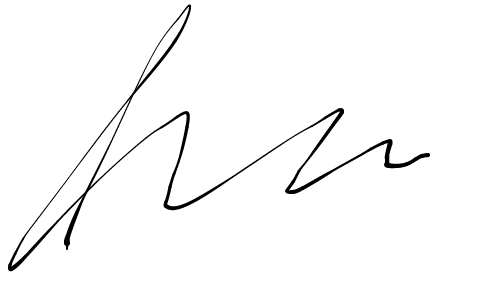
\includegraphics[width=0.35\textwidth]{unterschrift}\vspace*{-0.35cm}
					\\
					\rule[0.5ex]{12em}{0.55pt} & \rule[0.5ex]{12em}{0.55pt} \\
					(Ort, Datum) & (Eigenhändige Unterschrift)
					\\
				\end{tabular*} \\
			\end{table}

\end{document}